% What we did
In this experiment, we compute errors in estimated orientation for different features and regressors in order to determine the best combination for the retinogram dataset. To account for any bias introduced by an uneven distribution of thickness or contrast over the vessel set, we also investigate orientation error with respect to these image properties. This is important in this application since we are particularly interested in measuring the properties of the thinnest and faintest vessels.

In the following experiments, 200\,000 training pairs were taken from pixels that were known (from the ground truth segmentation) to lie on a vessel; the orientation of background pixels was not defined in this work.

To compare the performance of different features and regressors, we generated the cumulative distribution function over error (\fref{f:retina_graphs}a) and summarised performance by the median\footnote{The median is more robust than the mean to outliers in the error distribution.} errors over both the whole vessel and over the centre line only (\tref{t:retinopathy}).

We define ground truth orientation, at the vessel centres by skeletonising the masks and computing a locally linear fit; we then assign to every vessel pixel the orientation of its nearest centreline pixel.
\comment{Is this a reasonable proxy for true orientation?}

As a preprocessing step, we transformed all images to monochrome via a weighted sum of the three RGB channels (this proved marginally more successful than extracting features from all or any of the channels individually).

\comment{How can we justify throwing away two thirds of the available data? What were the weights? How much more successful was this? Is the difference significant?}

When sampling pixels with which to form the training data, we selected 200\,000 vessel pixels randomly over the set of training images. At every selected pixel, we then paired the chosen filter responses with the corresponding ground truth orientation, $t_{gt}$.

\comment{Why 200k points? Was this limit dictated by system requirements? What effect does the number of points have? (Try halving and doubling the number)}




\begin{figure}
\centering
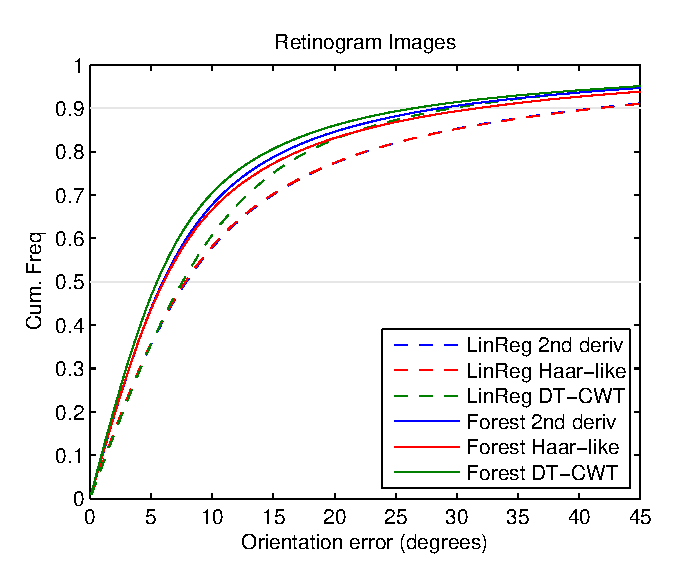
\includegraphics[width=0.48\columnwidth]{\figpath/retina/retinogram_expt}
%
\caption{Cumulative frequency of angular error for retinogram images.}
\label{f:cumfreq}
\end{figure} % from BMVC
\begin{figure}[t]
\centering
\def\figwidth{0.48\columnwidth}
\begin{tabular}{@{}c c@{}}
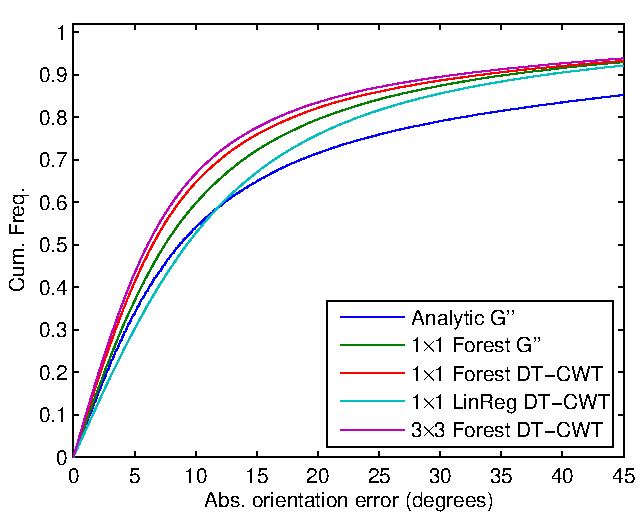
\includegraphics[width=\figwidth]{\figpath/retina/cumfreq} &
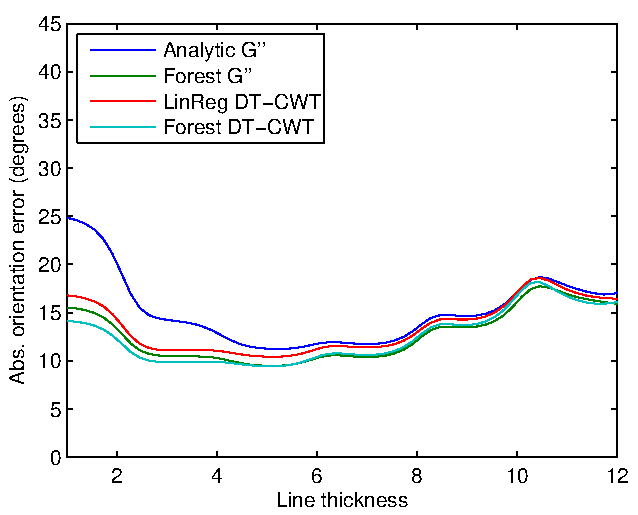
\includegraphics[width=\figwidth]{\figpath/retina/thickness_vs_error-summ} \\
(a) & (b)\\
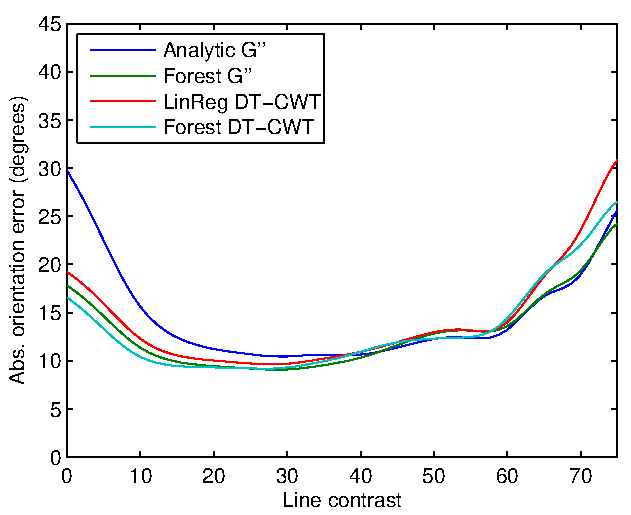
\includegraphics[width=\figwidth]{\figpath/retina/contrast_vs_error-summ} &
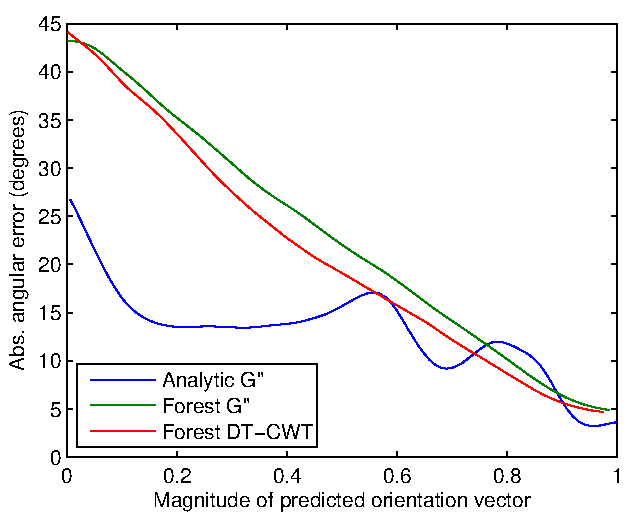
\includegraphics[width=\figwidth]{\figpath/retina/response_vs_error_ret} \\
(c) & (d)\\
\noalign{\smallskip}
\end{tabular}
%
\caption{Orientation estimation results for selected methods over pixels along the centre of the vessel: (a) Cumulative frequency of angular error; (b) Kernel estimate of mean error with respect to line thickness; (c) Kernel estimate of mean error with respect to line contrast; (d) Kernel estimate of mean error with respect to predicted orientation magnitude (for the analytic Gaussian, the absolute response scaled between 0 and 1 at the maximal angles is used).}
\label{f:retina_graphs}
\end{figure}

\comment{Some measure of spread for these figures, or a box plot to show significance.}
 % from MICCAI

% Discussions

\subsubsection{Choice of feature}
\label{s:exp_retinogram_orientation_wrt_feature}
% Compare all feature types with the most powerful and flexible regressor (e.g. Random Forests) so that complex feature types are not disadvantaged.

Features based on odd filters -- first derivatives of the Gaussian and the monogenic signal, for example -- were consistently outperformed by those that included even filters (\fref{f:retina_graphs}). This can be attributed to the high errors that occur when using only odd filters at the centre of a vessel where there is little or no image gradient; this failure is particularly acute for the most narrow vessels, consisting of a single pixel, where the whole vessel is a centreline by definition. 

Of the two features that use even filtering -- the second Gaussian derivatives and the \dtcwt{} -- the \dtcwt{} provided better estimates under most conditions. This suggests that using both odd and even filters (such that phase information becomes available) does indeed improve performance, though at a cost in computational demand.

%With the exception of the boosted regressor, the Haar-like approximation exhibited similar performance to the second derivative, suggesting that it may be used effectively in scenarios where efficiency is a concern.




\subsubsection{Choice of regressor}
\label{s:exp_retinogram_orientation_wrt_regressor}
% Compare all regressors with a given input feature (preferably the richest - dtcwt)
%
Comparing the performance of all estimation methods for a fixed input feature type (the \dtcwt{}), orientation was consistently estimated more accurately by regression compared to the analytic method with particular improvement seen in faint narrow vessels. 

Moreover, complex regressors such as Random Forests outperformed simpler ones such as linear regression. This suggests that the relationship between responses to the \dtcwt{} and line orientation is nonlinear.

Our use of statistical learning approaches was motivated threefold: by their ability to pool over scales and local neighbourhoods; to combine filter responses where an analytic solution was not obvious (when using the \dtcwt{}, for example); and to model data-dependent properties such as image noise and the observed distribution of line widths and contrasts. 

% Linear regression
%As noted earlier, when using second derivative responses it is necessary to compute the responses at the two possible solutions to determine which is the correct one. Since the linear regressor minimizes the average error, however, it contains no mechanism for selecting the correct orientation and this is likely to be one reason for its poor performance relative to more sophisticated regressors such as the Random Forest.


\subsubsection{Effect of window size}
\label{s:exp_retinogram_orientation_wrt_window_size}
Pooling results over a local neighbourhood by stacking filter responses into a single vector also had a significant effect on error rates. This was particularly the case for features based on odd filter responses, since it reduces the effect of small gradients at the centre-line by pooling estimates from nearby pixels with stronger gradients and therefore better estimates.

We also note that second Gaussian derivatives can be closely approximated using finite differencing of a first Gaussian derivative. Therefore, a linear regression over first derivative responses at neighbouring pixels is able to replicate the errors of the method based on second derivatives.


\subsubsection{Effects of line thickness}
\label{s:exp_retinogram_orientation_wrt_width}
% Compute orientation errors for lines of different widths
%
Because narrow vessels are interesting but occupy a small proportion of the vessel map, here we provide a breakdown of orientation errors for lines of different widths. To estimate the vessel widths, we computed the distance transform of the known vessel mask and set the width at every vessel pixels to that of the nearest centreline pixel.

\begin{figure}[t]
\centering
\def\figwidth{0.75\columnwidth}
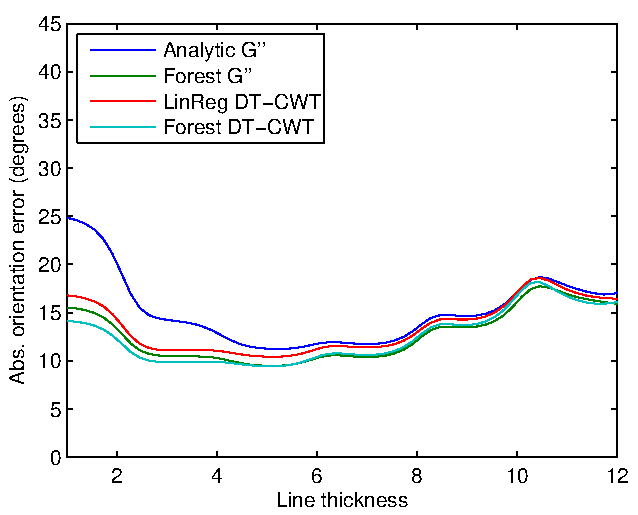
\includegraphics[width=\figwidth]{\figpath/retina/thickness_vs_error-summ} 
%
\caption{Orientation estimation results for selected methods over pixels along the centre of the vessel: Kernel estimate of mean error with respect to line thickness.}
\label{f:retinogram_orientation_wrt_width}
\end{figure}

We visualize this relationship using a one dimensional kernel smoother (\fref{f:retinogram_orientation_wrt_width}) and see that errors are similar for the thicker vessels (where there is more image information with which to estimate orientation and thus we expect all methods to perform well) but that the regression reduces error considerably for the narrower vessels. Interpreting results for vessels with a width of more than approximately 12 pixels is difficult because they are rare, which leads to high variability in the kernel estimate of error, and because the vessel width exceeds the central region of our largest filter. These vessels, however, are typically of less interest to the retinopathy community.


\subsubsection{Effects of line contrast}
To do so, we defined line contrast as the absolute difference between the vessel intensity and the mean intensity of background pixels in a $15{\times}15$ neighbourhood.

We see a similar effect when considering the distribution of error with respect to line contrast (\fref{f:retina_graphs}c): the learnt regressors outperform analytic methods especially on lines with low contrast though there is little significant difference between the methods for vessels of greater contrast. We also see errors begin to increase beyond a certain contrast, though this is most likely due again to the rarity of high contrast vessels and the correlation of high contrast with large width.

% We conclude that...?
Overall, combining \dtcwt{} features with Random Forest regression was most successful with the \dtcwt{} in particular benefiting from the improvement of Random Forests over simple linear regression (\tref{t:retinopathy})
